\section{Auswertung}
\label{sec:Auswertung}

% \begin{figure}
%   \centering
%   \includegraphics{plots/plot.pdf}
%   \caption{Plot.}
%   \label{fig:plot}
% \end{figure}



% \begin{table}
%    % Notation :  {% nicht entfernen ist sehr wichtig sonst Fehler !!
% \parbox{0.48\textwidth}{% %Ermöglicht zwei Tabellen neben einander
%   \centering
%   \sisetup{round-mode = places , round-precision = 0,scientific-notation=fixed, fixed-exponent = 0}
%          %rundet Werte aus Stelle, Stelle = ,  macht einen bestimmten festen exponenten
%   \resizebox{\textwidth}{!}{%  % skaliert zu große Tabellen
%   \begin{tabular}{S@{${}\pm{}$} S} % fügt plus minus Fehler Schreibweise hinzu
%     \toprule
%      $\text{e}_b / \si{\milli\meter}$ &
%      $\text{d}_b /\si{\milli\meter} $ & $\text{f}_b / \si{\milli\meter} $\\
%     \midrule
%     \bottomrule
%   \end{tabular}
%   % }
%   \caption{Tabellenunterschrift}
%   \label{tab:tab}
% }
% % \end{table}
% % \begin{table}
% \parbox{0.48\textwidth}{%
%   \centering
%   \sisetup{round-mode = places , round-precision = 0,scientific-notation=fixed, fixed-exponent = 0}
%   % \resizebox{\textwidth}{!}{%
%   \begin{tabular}{S@{${}\pm{}$} S}
%     \toprule
%      $\text{e}_b / \si{\milli\meter}$ &
%      $\text{d}_b /\si{\milli\meter} $ & $\text{f}_b / \si{\milli\meter} $\\
%     \midrule
%     \bottomrule
%   \end{tabular}
%   % }
%   \caption{Tabellenunterschrift}
%   \label{tab:tab}
% }
% \end{table}
\subsection{Hysterese Kurve des Magnetfeldes}
Die Feldstärke $B$ wird gegen den Feldstrom $I$, in Abbildung \ref{fig:BFeldplot}, aufgetragen. 
Das ermöglicht später das Magnetfeld zu berechnen, bei dem die Aufspaltung der Spektrallinien 
zu beobachten ist. In der Abbildung wird durch den linearen Teil der aufsteigenden Hysteresekurve eine 
Ausgleichsgerade gelegt. Die abfallende Hysteresekurve wurde zur Vollständigkeit gemessen und 
eingetragen. Die Ausgleichsrechnung wird mit Hilfe von \cite{scipy} und der Funktion
\begin{equation*}
B\left(I\right) = a \cdot I + b
\end{equation*}
durchgeführt.  Daraus ergibt sich $ a = \SI{61.7(4)}{\milli\tesla\per\ampere}$ und 
$ b = \SI{9(3)}{\milli\tesla}$. Die in Abbildung \ref{fig:BFeldplot} schwarz markierten Werte wurden 
in der Ausgleichsrechnung nicht betrachtet, da diese nicht mehr im linearen Teil der Hysteresekurve 
liegen.
\begin{figure}
  \centering
  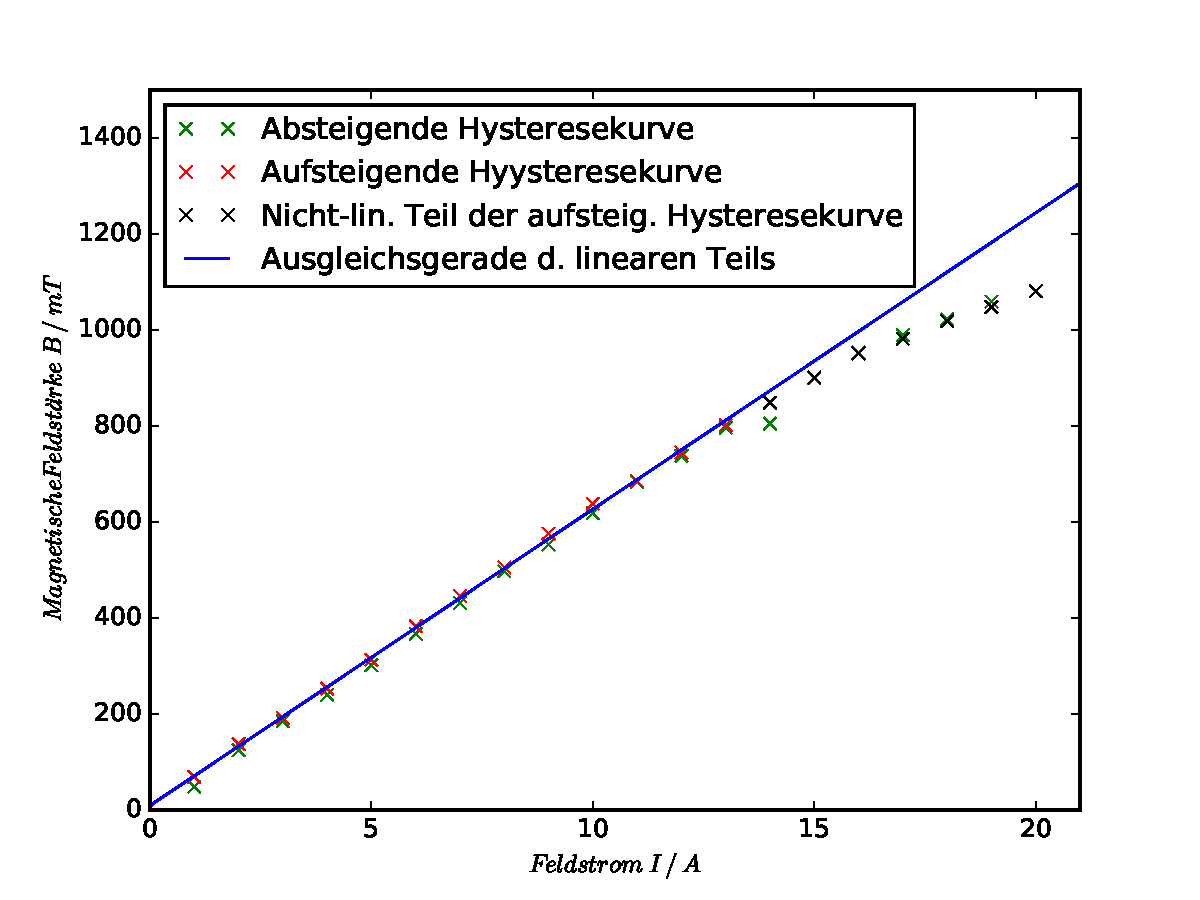
\includegraphics[height = 7cm]{plots/BFeldplot.pdf}
  \caption{Auf- und absteigende Hysterese Kurve des Magnetfeldes mit Ausgleichsgerade für den linearen Teil.}
   \label{fig:BFeldplot}
\end{figure}
\FloatBarrier

\subsection{Methode zur Auswertung des Bildmaterials}
\label{sec:MB}
Das Bildmaterial wurde zuerst mit \textit{Fiji} \cite{fiji} ausgewertet, indem ein 
Intensitätsdiagram 
erstellt wurde, diese sind in den Abbildungen \ref{fig:p1},\ref{fig:p2}, \ref{fig:p3}, 
\ref{fig:p4}, \ref{fig:p5} und \ref{fig:p6} zu betrachten. Anschließend wurde aus den Plots die 
Position der Intensitätsmaxima ausgelesen. Der Abstand zwischen diesen Maxima wird dann $\Delta s$ 
oder $\delta s$ bei Aufspaltung eines Maximums bezeichnet.


\subsection{Methoden zur Bestimmung der Übergangsenergie, der Wellenlängenänderung \texorpdfstring{$\delta \lambda$}{math} und des Übergangs-Landre-Faktors}
\label{sec:MR}


Der Zusammenhang zwischen der Wellenlänge $\lambda$ und Wellenlängenänderung $\delta \lambda$ und 
dem Gangunterschied $\Delta s$ und der Aufspaltung $\delta s$ ist gegeben durch \cite{Anleitung}:
\begin{equation}
\delta \lambda = \frac{1}{2} \frac{\delta s}{\Delta s} \cdot \Delta \lambda_D \; .
\label{eq:DL}
\end{equation}
Dabei bezeichnet $\Delta \lambda_D$ das Dispersionsgebiet der Lummer-Gehrcke-Platte mit 
\begin{equation*}
\Delta \lambda_D = \frac{\lambda^2}{2\cdot d} \cdot \sqrt{\frac{1}{n^2 -1}} \; ,
\label{eq:dell}
\end{equation*}
dabei ist $d = \SI{4}{\milli\meter}$, $n(\SI{644}{\nano\meter}) = 1.4567$ und 
$n(\SI{480}{\nano\meter}) = 1.4635$. 
Nun wird die Energie des ausgesandten Lichtes betrachtet, um später auf die Energie der Aufspaltung 
zu schließen. Die Energie des Lichtes ist gegeben durch $E = \sfrac{\symup{hc}}{\lambda}$, die 
Energie der Aufspaltung ist die Differenz der Energie $\Delta E$ vor und nach der Aufspaltung, also 
der Wellenlängenänderung $\delta \lambda$. Dann folgt:
\begin{equation*}
E\left(\lambda + \delta \lambda\right) \stackrel{\text{Taylor}}{\approx} 
E(\lambda) + \frac{\partial E(\lambda + \delta \lambda)}{\partial \lambda}  \biggr \rvert_{\lambda + \delta 
\lambda = \lambda } \cdot\delta \lambda = E(\lambda) - \frac{\symup{hc}}{\lambda^2}\delta \lambda
 \; . 
\label{eq:dE}
\end{equation*}
Dann folgt  
\begin{equation}
\Delta E = E(\lambda + \delta \lambda ) - E( \lambda) = - \frac{hc}{\lambda^2} \delta \lambda \; .
\end{equation}
Daraus ergibt sich mit der Gleichung \eqref{eq:Egij} 
\begin{equation}
\lvert g_{ij} \rvert = \frac{hc}{\lambda^2} \frac{1}{\mu_B B_z} \delta \lambda \; .
\label{eq:gij}
\end{equation} 
Für die folgenden Ergebnisse kann nun $\delta \lambda$, $\Delta E$ und $\lvert g_{ij} \rvert$ 
bestimmt werden.

\subsection{Zeeman-Effekt beim Übergang von \texorpdfstring{${}^1\symup{P}_1 \iff {}^1 \symup{D}_2$}{math} in Cadmium (\texorpdfstring{$\lambda= \SI{643.8}{\nano\meter}$}{math})}
Wie im Abschnitt \ref{sec:MB} zuvor besprochen wurden Intensitätsdiagramme erstellt und daraus die 
Positionen der Maxima bestimmt, um daraus auf den Gangunterschied $\Delta s$ und die Aufspaltung 
$\delta s$ zu schließen. Die Intensitätsdiagramme sind in den Abbildungnen \ref{fig:p1} und 
\ref{fig:p2} zu betrachten. Das Bildmaterial aus dem Versuch ist in der Abbildung 
\ref{fig:rot} zu betrachten. Die so ermittelten Werte sind in den Tabellen \ref{tab:trp}, 
\ref{tab:trDs} und \ref{tab:trpds} dargestellt. Für $\lambda = \SI{643.8}{\nano\meter}$ 
ergibt sich für das Dispersionsgebiet $\Delta\lambda_D = 4.89\cdot10^{-11}$. Anhand der Gleichungen 
\begin{equation}
\bar{\Delta s } = \frac{1}{N} \sum_{j=1} ^N \Delta s_j 
\qquad \text{mit der Unsicherheit} \qquad
\sigma = \sqrt{\frac{1}{N(N-1)} \sum_{j=1} ^N (\Delta s_j - \bar{\Delta s})^2} \; ,
\label{eq:mittel}
\end{equation}
wird der mittelere Gangunterschied $ \bar{\Delta s} = \SI{336(6)} \symup{px}$ und die mittlere 
Aufspaltung $\bar{\delta s} = \SI{158(3)}\symup{px}$. Daraus ergibt sich dann mit der Gleichung 
\eqref{eq:dell} die Wellenlängenänderung $\delta \lambda = \SI{115(3)}{\nano\meter}$, damit folgt 
dann $\Delta E = \SI{3.45(9)e-05}{\eV} $ und mit der Gleichung \ref{eq:gij} 
$ \lvert g_{ij} \rvert = \SI{1.00(3)}{} $. Der Übergang mit dem $\pi$-polarsiertem Licht war, wie 
erwartet, nicht zu beobachten. 




\begin{figure}
\centering
\begin{subfigure}{0.48\textwidth}
  \centering
  
\includegraphics[height=5cm]{pics/644nm_B=0_P=0.JPG}
  \caption{Ohne Magnetfeld.}
  \label{fig:roto}
\end{subfigure}
\begin{subfigure}{0.48\textwidth}
  \centering
  
\includegraphics[height=5cm]{pics/644nm_I=9.5A_P=0.JPG}
  \caption{Mit Magnetfeld \texorpdfstring{$B = \SI{596(2)}{\milli\tesla}$}{math}.}
  \label{fig:rotb}
\end{subfigure}
\caption{Spektrallinie des \texorpdfstring{${}^1\symup{P}_1 \iff {}^1 \symup{D}_2$}{math} Übergangs.}
\label{fig:rot}
\end{figure}


\begin{figure}
  \centering
  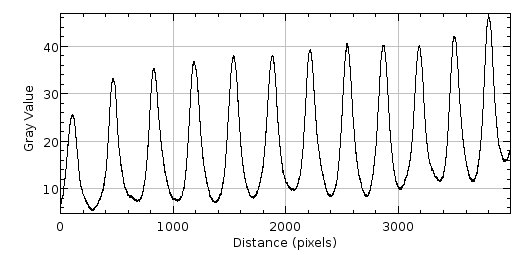
\includegraphics[height=5cm]{pics/Plot_644nm_B=0_P=0.jpg}
  \caption{Intensitätsdiagram zum Bildmaterial in Abbildung \ref{fig:roto}.}
  \label{fig:p1}
\end{figure}

\begin{figure}
  \centering
  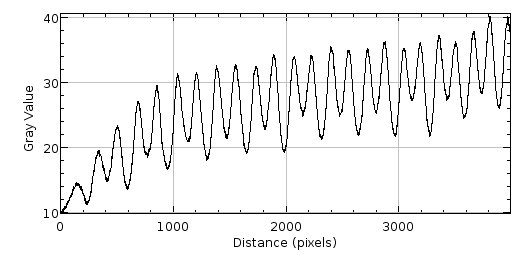
\includegraphics[height=5cm]{pics/Plot_644nm_I=9.5A_P=0.jpg}
  \caption{Intensitätsdiagram zum Bildmaterial in Abbildung \ref{fig:rotb}.}
  \label{fig:p2}
\end{figure}

\begin{table}
  \centering
  \sisetup{round-mode = places , round-precision = 0,scientific-notation=fixed, fixed-exponent = 0}
  \begin{tabular}{S} 
    \toprule
    $\text{Position der Intensitätsmaxima} / \symup{px} $\\
    \midrule
      1.090000000000000000e+02\\
      4.680000000000000000e+02\\
      8.310000000000000000e+02\\
      1.186000000000000000e+03\\
      1.536000000000000000e+03\\
      1.883000000000000000e+03\\
      2.217000000000000000e+03\\
      2.542000000000000000e+03\\
      2.868000000000000000e+03\\
      3.185000000000000000e+03\\
      3.494000000000000000e+03\\
      3.803000000000000000e+03\\
    \bottomrule
  \end{tabular}
  \caption{Positionen der Intensitätsmaxima vom Bildmaterial in Abbildung \ref{fig:roto}.}
  \label{tab:trp}
\end{table}
\begin{table}
  \centering 
  \sisetup{round-mode = places , round-precision = 0,scientific-notation=fixed, fixed-exponent = 0}
  \begin{tabular}{S}
    \toprule
     $\text{Gangunterschied}\; \Delta s / \symup{px} $\\
    \midrule
      3.590000000000000000e+02\\
      3.630000000000000000e+02\\
      3.550000000000000000e+02\\
      3.500000000000000000e+02\\
      3.470000000000000000e+02\\
      3.340000000000000000e+02\\
      3.250000000000000000e+02\\
      3.260000000000000000e+02\\
      3.170000000000000000e+02\\
      3.090000000000000000e+02\\
      3.090000000000000000e+02\\
    \bottomrule
  \end{tabular}
  \caption{Gangunterschiede im Bildmaterial aus Abbildung \ref{fig:roto} 
           berechnet aus den Werten aus Tabelle \ref{tab:trp}.}
  \label{tab:trDs}
\end{table}

\begin{table}
  \centering
  \sisetup{round-mode = places , round-precision = 0,scientific-notation=fixed, fixed-exponent = 0}
  \begin{tabular}{S S S}
    \toprule
     \multicolumn{2}{c}{$\text{Postion der Aufspaltungsmaxima} /\symup{px} $} 
     & $\text{Aufspaltung}\; \delta s /\symup{px}  $\\
    \midrule
      3.380000000000000000e+02 & 5.080000000000000000e+02 & 1.700000000000000000e+02\\
      6.920000000000000000e+02 & 8.560000000000000000e+02 & 1.640000000000000000e+02\\
      1.041000000000000000e+03 & 1.207000000000000000e+03 & 1.660000000000000000e+02\\
      1.387000000000000000e+03 & 1.556000000000000000e+03 & 1.690000000000000000e+02\\
      1.737000000000000000e+03 & 1.891000000000000000e+03 & 1.540000000000000000e+02\\
      2.073000000000000000e+03 & 2.225000000000000000e+03 & 1.520000000000000000e+02\\
      2.391000000000000000e+03 & 2.556000000000000000e+03 & 1.650000000000000000e+02\\
      2.722000000000000000e+03 & 2.879000000000000000e+03 & 1.570000000000000000e+02\\
      3.046000000000000000e+03 & 3.190000000000000000e+03 & 1.440000000000000000e+02\\
      3.346000000000000000e+03 & 3.506000000000000000e+03 & 1.600000000000000000e+02\\
      3.670000000000000000e+03 & 3.811000000000000000e+03 & 1.410000000000000000e+02\\
    \bottomrule
  \end{tabular}
  \caption{Postion der Aufspaltungsmaxima im Bildmaterial aus Abbildung \ref{fig:rotb} und die daraus resultierende Aufspaltung.}
  \label{tab:trpds}
\end{table}


\FloatBarrier




\subsection{Zeeman-Effekt beim Übergang von \texorpdfstring{${}^3\symup{S}_1 \iff {}^3 \symup{P}_2$}{math} in Cadmium (\texorpdfstring{$\SI{480}{\nano\meter}$}{math})}
Durch die Methoden die im Abschnitt \ref{sec:MB} besprochen wurden, ergeben sich die Abbildungen 
\ref{fig:p3}, \ref{fig:p4}, \ref{fig:p5} und \ref{fig:p6}. Daraus ergeben sich wiederum die 
Wertetabellen \ref{tab:t3p}, \ref{tab:t3Ds}, \ref{tab:t4}, \ref{tab:t5p}, \ref{tab:t5Ds} und  
\ref{tab:t6}. Die Bildmaterialen zu den Intensitätsdiagrammen und den Werten sind in den Abbildungen 
\ref{fig:bp0}, \ref{fig:bp0b}, \ref{fig:bp90} und \ref{fig:bp90b} abgebildet. 
\newline 
An dieser Stelle danken wir \textit{Laura Kodytek} für die freundliche Bereitstellung der 
Bildmaterialien aus Abbildung \ref{fig:bp90} und \ref{fig:bp90b}, da es uns nicht möglich war den 
Übergang mit $\pi$-Polarisation mit hinreichend großer Aufspaltung zu beobachten.
\newline 
Die folgenden Ergebnisse wurden mit den Methoden aus Abschnitt \ref{sec:MR} berechnet, für beide 
Polarisationen wurde mit der Gleichung \eqref{eq:DL} $ \Delta \lambda_D = \SI{2.69e-11}{\meter}$ 
bestimmt. 
\paragraph{\texorpdfstring{$\sigma$}{math}-Polarisation}
Aus den Werten aus Tabelle \ref{tab:t3Ds} folgt dann mit den Formeln \eqref{eq:mittel} der mittlere 
Gangunterschied $\bar{\Delta s} = \SI{319(13)}\symup{px}$ und mit den Werten aus Tabelle 
\ref{tab:t4} die mittlere Aufspaltung $\delta s = \SI{125(10)} \symup{px}$. Daraus ergibt sich dann 
$\delta \lambda = \SI{5.3(5)}{\pico\meter}$ und es folgt $\Delta E = \SI{2.8(3)e-5}{\eV}$ und 
$\lvert g_{ij} \rvert = \SI{1.4(1)}{}$. 


\begin{figure}[h!]
 \centering 
 \begin{subfigure}{0.48\textwidth}
  \centering
  
\includegraphics[height=5cm]{pics/480nm_B=0_P=0.JPG}
  \caption{Ohne Magnetfeld.}
  \label{fig:bp0}
 \end{subfigure}
 \begin{subfigure}{0.48\textwidth}
  \centering
  
\includegraphics[height=5cm]{pics/480nm_I=5.5_P=0.JPG}
  \caption{Mit Magnetfeld \texorpdfstring{$B = \SI{348(2)}{\milli\tesla}$}{math}.}
  \label{fig:bp0b}
 \end{subfigure}
 \caption{Spektrallinie des \texorpdfstring{${}^3\symup{S}_1 \iff {}^3 \symup{P}_2$}{math} Übergangs}
 \label{fig:BP0}
\end{figure}

\begin{figure}[h!]
  \centering
  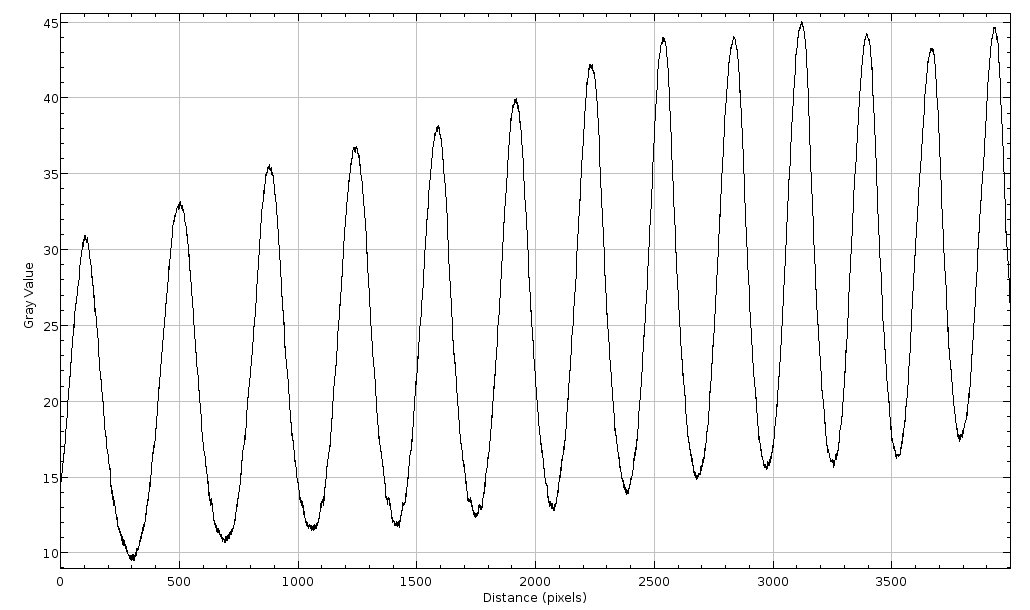
\includegraphics[height=5cm]{pics/Plot_480nm_B=0_P=0.jpg}
  \caption{Intensitätsdiagram zum Bildmaterial in Abbildung \ref{fig:bp0}.}
  \label{fig:p3}
\end{figure}
\begin{figure}[h!]
  \centering
  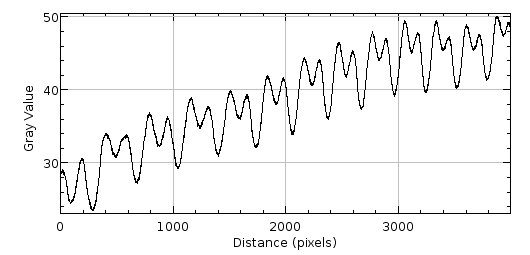
\includegraphics[height=5cm]{pics/Plot_480nm_I=5.5_P=0.jpg}
  \caption{Intensitätsdiagram zum Bildmaterial in Abbildung \ref{fig:bp0b}.}
  \label{fig:p4}
\end{figure}

\begin{table}[h!]
  \centering
  \sisetup{round-mode = places , round-precision = 0,scientific-notation=fixed, fixed-exponent = 0}
  \begin{tabular}{S} 
    \toprule
    $\text{Position der Intensitätsmaxima} / \symup{px} $\\
    \midrule
      1.090000000000000000e+02\\
      4.680000000000000000e+02\\
      8.310000000000000000e+02\\
      1.186000000000000000e+03\\
      1.536000000000000000e+03\\
      1.883000000000000000e+03\\
      2.217000000000000000e+03\\
      2.542000000000000000e+03\\
      2.868000000000000000e+03\\
      3.185000000000000000e+03\\
      3.494000000000000000e+03\\
      3.803000000000000000e+03\\
    \bottomrule
  \end{tabular}
  \caption{Positionen der Intensitätsmaxima vom Bildmaterial in Abbildung \ref{fig:bp0}.}
  \label{tab:t3p}
\end{table}
\begin{table}
  \centering
  \sisetup{round-mode = places , round-precision = 0,scientific-notation=fixed, fixed-exponent = 0}
  \begin{tabular}{S}
    \toprule
     $\text{Gangunterschied}\; \Delta s / \symup{px} $\\
    \midrule
      3.590000000000000000e+02\\
      3.630000000000000000e+02\\
      3.550000000000000000e+02\\
      3.500000000000000000e+02\\
      3.470000000000000000e+02\\
      3.340000000000000000e+02\\
      3.250000000000000000e+02\\
      3.260000000000000000e+02\\
      3.170000000000000000e+02\\
      3.090000000000000000e+02\\
      3.090000000000000000e+02\\
    \bottomrule
  \end{tabular}
  \caption{Gangunterschied im Bildmaterial aus Abbildung \ref{fig:bp0}, berechnet aus den Werten aus Tabelle \ref{tab:t3p}.}
  \label{tab:t3Ds}
\end{table}

\begin{table}[h!]
  \centering
  \sisetup{round-mode = places , round-precision = 0,scientific-notation=fixed, fixed-exponent = 0}
  \begin{tabular}{S S S}
    \toprule
     \multicolumn{2}{c}{$\text{Postion der Aufspaltungsmaxima} /\symup{px} $} 
     & $\text{Aufspaltung}\; \delta s /\symup{px}  $\\
    \midrule
      3.380000000000000000e+02 & 5.080000000000000000e+02 & 1.700000000000000000e+02\\
      6.920000000000000000e+02 & 8.560000000000000000e+02 & 1.640000000000000000e+02\\
      1.041000000000000000e+03 & 1.207000000000000000e+03 & 1.660000000000000000e+02\\
      1.387000000000000000e+03 & 1.556000000000000000e+03 & 1.690000000000000000e+02\\
      1.737000000000000000e+03 & 1.891000000000000000e+03 & 1.540000000000000000e+02\\
      2.073000000000000000e+03 & 2.225000000000000000e+03 & 1.520000000000000000e+02\\
      2.391000000000000000e+03 & 2.556000000000000000e+03 & 1.650000000000000000e+02\\
      2.722000000000000000e+03 & 2.879000000000000000e+03 & 1.570000000000000000e+02\\
      3.046000000000000000e+03 & 3.190000000000000000e+03 & 1.440000000000000000e+02\\
      3.346000000000000000e+03 & 3.506000000000000000e+03 & 1.600000000000000000e+02\\
      3.670000000000000000e+03 & 3.811000000000000000e+03 & 1.410000000000000000e+02\\
    \bottomrule
  \end{tabular}
  \caption{Position der Aufspaltungsmaxima im Bildmaterial aus Abbildung \ref{fig:bp0b} und die daraus resultierende Aufspaltung.}
  \label{tab:t4}
\end{table}


\FloatBarrier

\paragraph{\texorpdfstring{$\pi$}{math}-Polarisation}
Aus den Werten von Tabelle \ref{tab:t5Ds} foglt der mittlere Gangunterschied 
$\bar{\Delta s} = \SI{400(40)}{} \symup{px}$ und mit den Werten aus Tabelle \ref{tab:t6} folgt 
$ \bar{\delta s} = \SI{128(13)}{}\symup{px}$. Damit ist dann 
$\delta \lambda = \SI{4.3(6)}{\pico\meter} $ und somit $\Delta E = \SI{2.3(3)}{\eV}$ und 
$\lvert g_{ij} \rvert = \SI{1.4(1)}{}$.




\begin{figure}[h!]
 \begin{subfigure}{0.48\textwidth}
  \centering
  
\includegraphics[height=5cm]{pics/04_480nm_B=0.JPG}
  \caption{Ohne Magnetfeld.}
  \label{fig:bp90}
 \end{subfigure}
 \begin{subfigure}{0.48\textwidth}
  \centering
  \includegraphics[height=5cm]{pics/06_480nm_B=0,981_Pol=90°.JPG}
  \caption{Mit Magnetfeld \texorpdfstring{$B = \SI{981}{\milli\tesla}$}{math}.}
\label{fig:bp90b}
 \end{subfigure}
\caption{Spektrallinie des \texorpdfstring{${}^3\symup{S}_1 \iff {}^3 \symup{P}_2$}{math} Übergangs}
\end{figure}

\begin{figure}[h!]
  \centering
  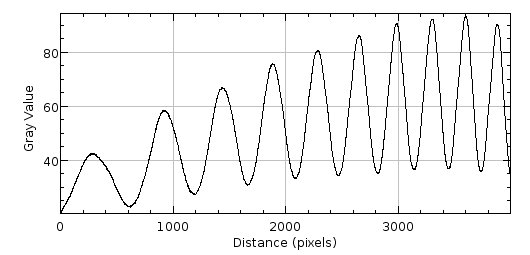
\includegraphics[height=5cm]{pics/Plot_480nm_B=0.jpg}
  \caption{Intensitätsdiagram zum Bildmaterial in Abbildung \ref{fig:bp90}.}
  \label{fig:p5}
\end{figure}
\begin{figure}[h!]
  \centering
  \includegraphics[height=5cm]{pics/Plot_06_480nm_B=0,981_Pol=90°.jpg}
  \caption{Intensitätsdiagram zum Bildmaterial in Abbildung \ref{fig:bp90b}.}
  \label{fig:p6}
\end{figure}

\begin{table}[h!]
  \centering
  \sisetup{round-mode = places , round-precision = 0,scientific-notation=fixed, fixed-exponent = 0}
  \begin{tabular}{S} 
    \toprule
    $\text{Position der Intensitätsmaxima} / \symup{px} $\\
    \midrule
      1.090000000000000000e+02\\
      4.680000000000000000e+02\\
      8.310000000000000000e+02\\
      1.186000000000000000e+03\\
      1.536000000000000000e+03\\
      1.883000000000000000e+03\\
      2.217000000000000000e+03\\
      2.542000000000000000e+03\\
      2.868000000000000000e+03\\
      3.185000000000000000e+03\\
      3.494000000000000000e+03\\
      3.803000000000000000e+03\\
    \bottomrule
  \end{tabular}
  \caption{Position der Intensitätsmaxima vom Bildmaterial in Abbildung \ref{fig:bp90}.}
  \label{tab:t5p}
\end{table}
\begin{table}
  \centering
  \sisetup{round-mode = places , round-precision = 0,scientific-notation=fixed, fixed-exponent = 0}
  \begin{tabular}{S}
    \toprule
     $\text{Gangunterschied}\; \Delta s / \symup{px} $\\
    \midrule
     6.340000000000000000e+02\\
     5.140000000000000000e+02\\
     4.480000000000000000e+02\\
     4.030000000000000000e+02\\
     3.630000000000000000e+02\\
     3.320000000000000000e+02\\
     3.220000000000000000e+02\\
     2.970000000000000000e+02\\
     2.770000000000000000e+02\\
    \bottomrule
  \end{tabular}
  \caption{Gangunterschied im Bildmaterial aus Abbildung \ref{fig:bp90}, berechnet aus den Werten aus Tabelle \ref{tab:t5p}.}
  \label{tab:t5Ds}
\end{table}

\begin{table}[h!]
  \centering
  \sisetup{round-mode = places , round-precision = 0,scientific-notation=fixed, fixed-exponent = 0}
  \begin{tabular}{S S S}
    \toprule
     \multicolumn{2}{c}{$\text{Postion der Aufspaltungsmaxima} /\symup{px} $} 
     & $\text{Aufspaltung}\; \delta s /\symup{px}  $\\
    \midrule
      3.380000000000000000e+02 & 5.080000000000000000e+02 & 1.700000000000000000e+02\\
      6.920000000000000000e+02 & 8.560000000000000000e+02 & 1.640000000000000000e+02\\
      1.041000000000000000e+03 & 1.207000000000000000e+03 & 1.660000000000000000e+02\\
      1.387000000000000000e+03 & 1.556000000000000000e+03 & 1.690000000000000000e+02\\
      1.737000000000000000e+03 & 1.891000000000000000e+03 & 1.540000000000000000e+02\\
      2.073000000000000000e+03 & 2.225000000000000000e+03 & 1.520000000000000000e+02\\
      2.391000000000000000e+03 & 2.556000000000000000e+03 & 1.650000000000000000e+02\\
      2.722000000000000000e+03 & 2.879000000000000000e+03 & 1.570000000000000000e+02\\
      3.046000000000000000e+03 & 3.190000000000000000e+03 & 1.440000000000000000e+02\\
      3.346000000000000000e+03 & 3.506000000000000000e+03 & 1.600000000000000000e+02\\
      3.670000000000000000e+03 & 3.811000000000000000e+03 & 1.410000000000000000e+02\\
    \bottomrule
  \end{tabular}
  \caption{Position der Aufspaltungsmaxima im Bildmaterial aus Abbildung \ref{fig:bp90b} und die daraus resultierende Aufspaltung.}
  \label{tab:t6}
\end{table}


\FloatBarrier







